\documentclass[a4paper, 10pt]{article}
\usepackage[english]{babel}
\usepackage[utf8]{inputenc}
\usepackage{enumitem}
\usepackage{float}
\usepackage{titlesec}
\usepackage{framed}
\usepackage{listings}
\usepackage{graphicx}
\usepackage{titling}
\usepackage{blindtext}
\usepackage{amsmath}  % for \hookrightarrow
\usepackage{xcolor}   % for \textcolor
\graphicspath{ {../ER/} }
\usepackage[hmargin=2cm,vmargin=3.5cm,bmargin=2cm]{geometry}

\setlist[itemize]{noitemsep, topsep=0pt}
\setlength\parindent{0pt}

\setcounter{secnumdepth}{0} %% no numbering

\begin{document}
\title{Advanced DataBases C4 Group\\\
  \huge Bank Management System}
\author{
  Samuel Lúcio Vicente, 251720
  \and
  Daniel Silva, 251702
  \and
  Jorge Marrero Camiruaga, 251438
}

\date{Politechnika Wrocławska\\today}

\maketitle

\lstset{
  basicstyle=\small\ttfamily,
  frame=lrtb,
  numbers=left,
  columns=fullflexible,
  breaklines=true,
  postbreak=\mbox{\textcolor{red}{$\hookrightarrow$}\space}
}

\section{Short Description}
This database models a bank with Accounts that can either be a SavingsAccount or a CurrentAccount. There are some operations that are permitted, Withdraw from the CurrentAccount, Transfer between accounts, Loan, Pay the loan, Deposit on Account. There are employees that work in a branch that have roles, this database tracks the history of all the employees on every branch, and the previous roles that some particular employee has had and which branch he has working at.

\section{ERD}
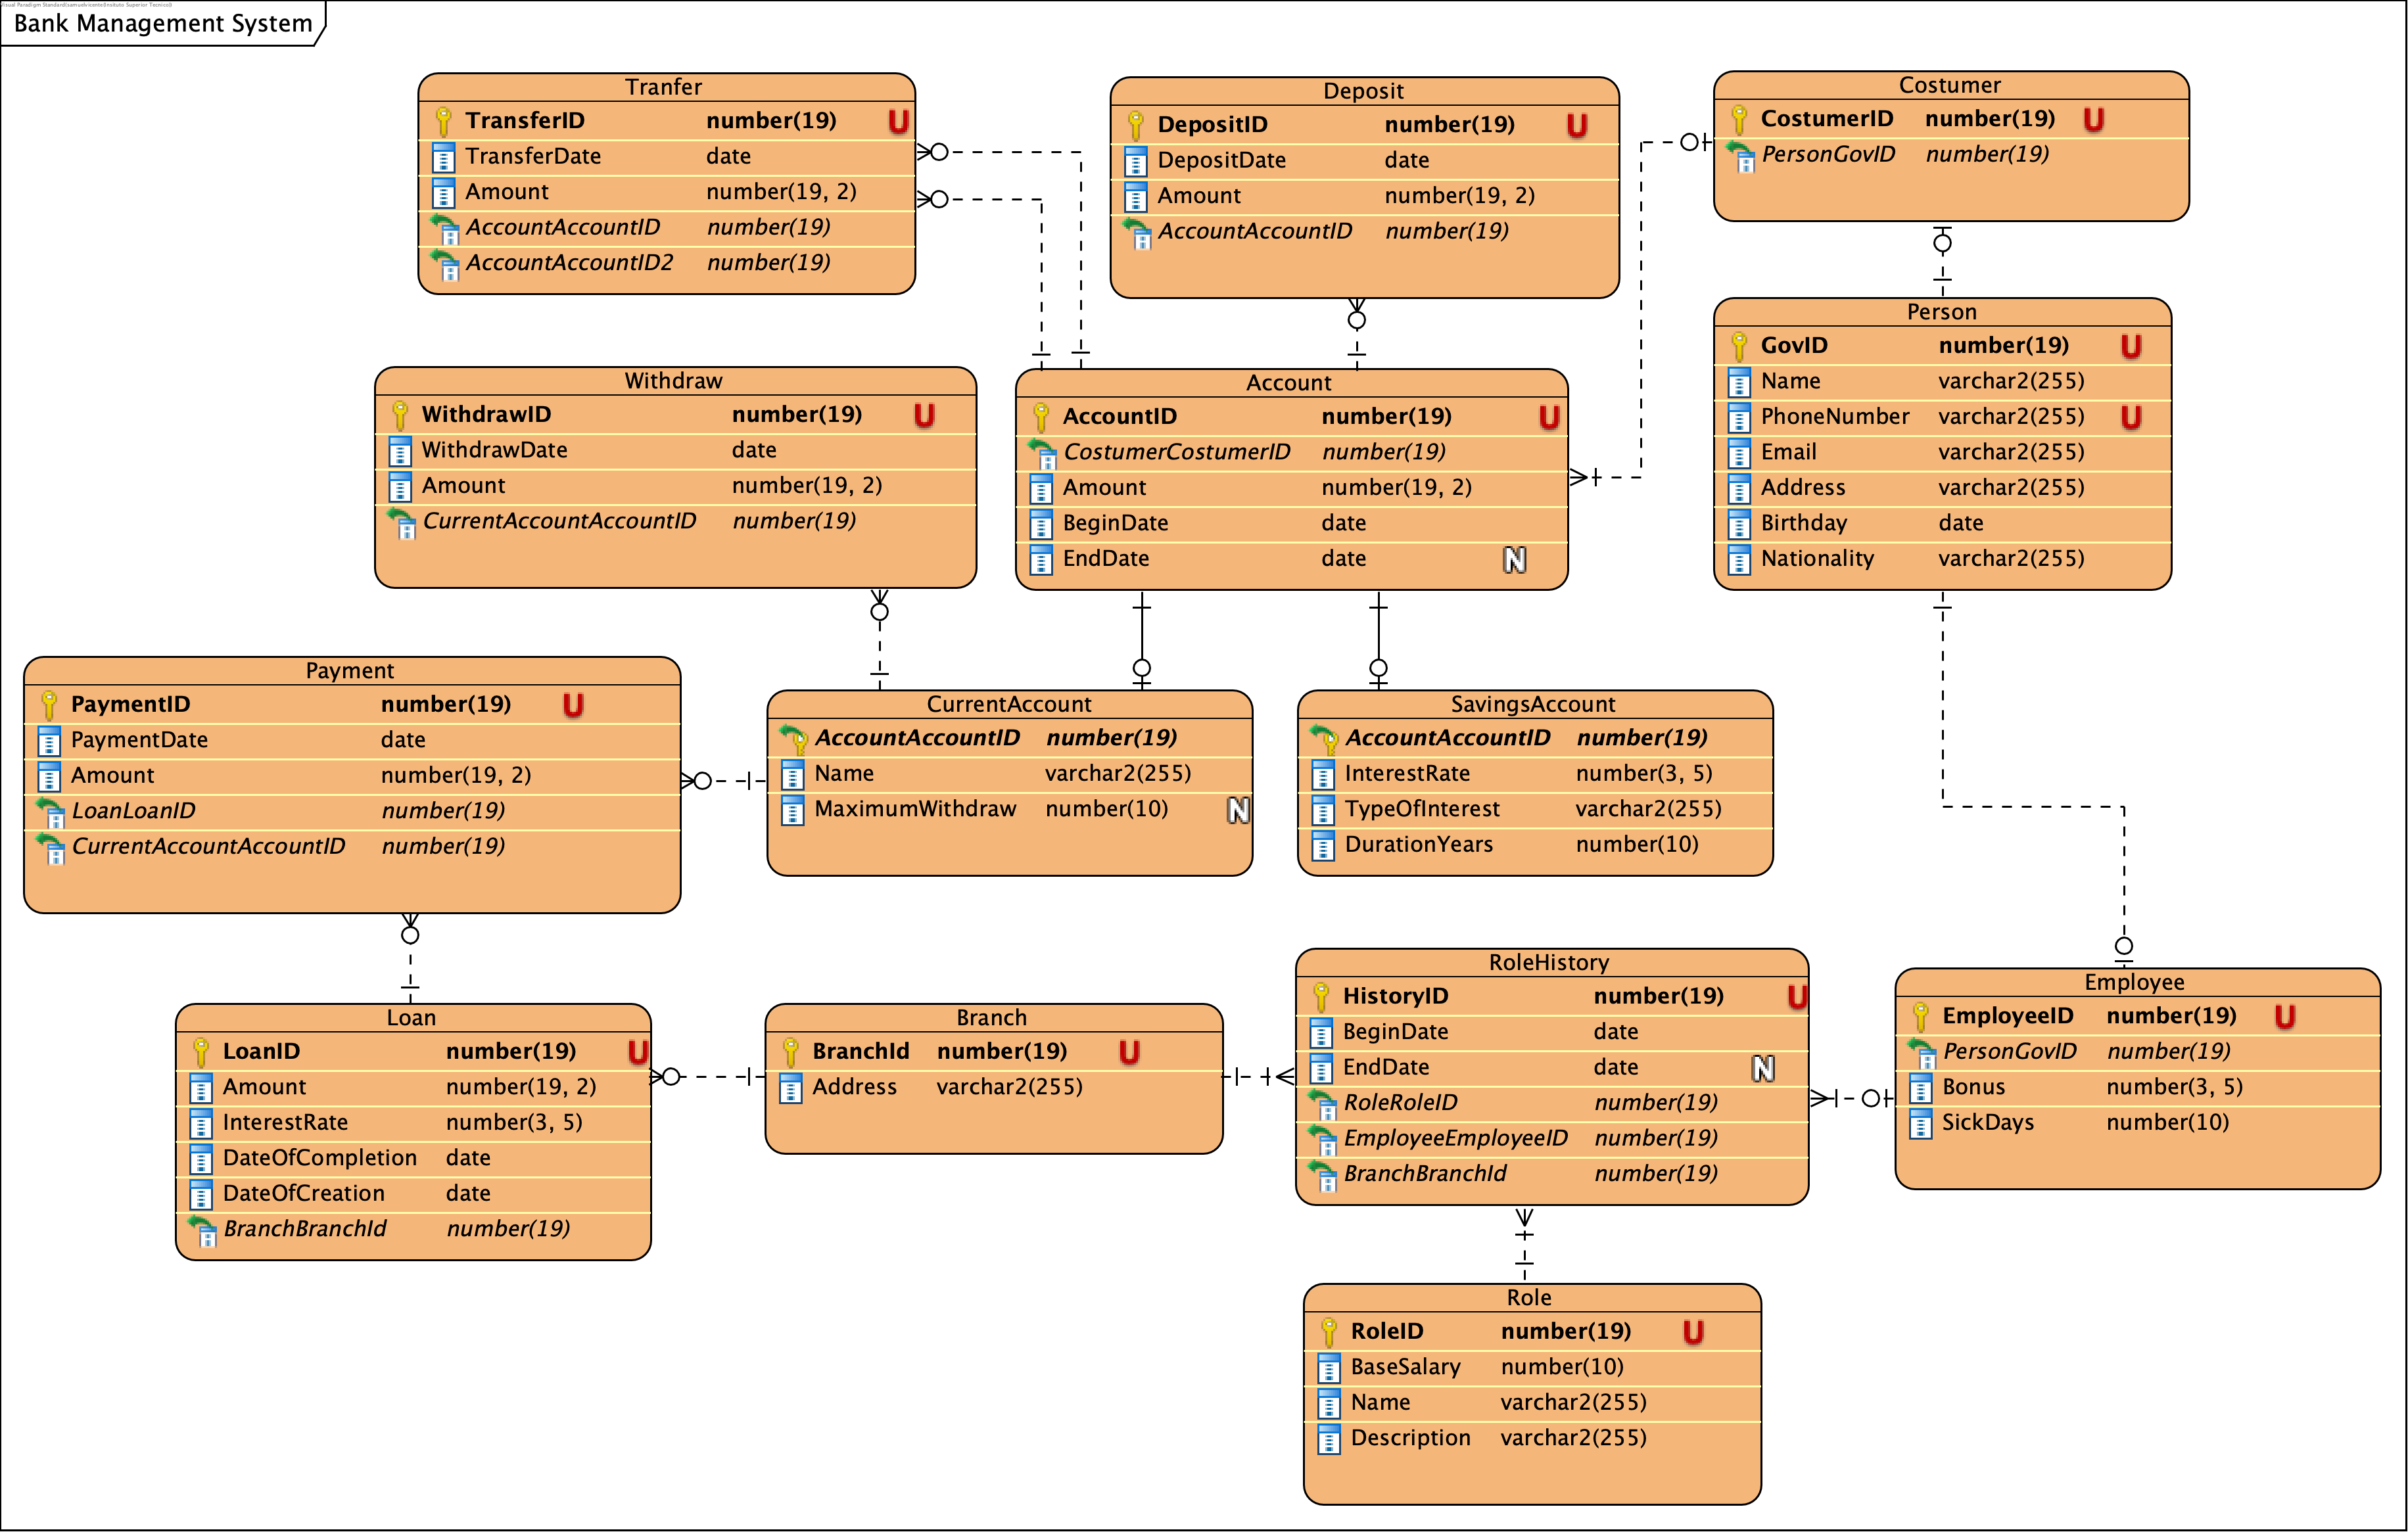
\includegraphics[width=\textwidth,height=\textheight,keepaspectratio]{bms}
\section{Generator Script}
\begin{lstlisting}[language=python]
import random
import math

def newDate(year, month, numeroMeses):
    newMonth=(month+numeroMeses)%12 if (month+numeroMeses)%12 != 0 else 12
    newYear=year + (math.floor(numeroMeses/12 +1) if month>newMonth else math.floor(numeroMeses/12))
    return (newYear, newMonth)
phoneNumber=900000000
govId=1111111111

loanID=1
costumerID=1
employeeID=1
branchID=1
accountID=1
with open("./resources/citiesCountries.txt", 'r', encoding='utf-8') as cities:
    places=cities.read().splitlines()
    with open("./resources/costumerNames.txt", 'r', encoding='utf-8') as costumerNames: 
        with open("./resources/employeeName.txt", 'r', encoding='utf-8') as employeeNames: 
            with open("./resources/Roles.txt", 'r', encoding='utf-8') as roles:
                #Create Roles
                for role in roles:
                    baseSalary=role.split(",")[1].strip()
                    name=role.split(",")[0].strip()
                    print(f"INSERT INTO Role(BaseSalary, Name) VALUES ({baseSalary}, '{name}');")
                #Finish Roles

                #create branch
                for place in places:
                    print(f"INSERT INTO Branch(Address) VALUES ('{place}');")
                    i=1
                    #create 8 employees per branch
                    beginDate=f"TO_DATE('{random.randint(1,28)}-{random.randint(1,12)}-{random.randint(2001,2018)}','DD-MM-YYYY')"
                    for name in employeeNames:
                        name=name.strip()
                        email=f"{name.strip().replace(' ', '_')}{random.randint(0,100)}@sapo.pt"
                        address=place
                        birthday=f"TO_DATE('{random.randint(1,28)}-{random.randint(1,12)}-{random.randint(1950,2000)}','DD-MM-YYYY')"
                        nationality=address.split(",")[1].strip()
                        print(f"INSERT INTO Person(GovID,Name, PhoneNumber, Email, Address, Birthday, Nationality) VALUES ({govId},'{name}','{phoneNumber}', '{email}', '{address}', {birthday}, '{nationality}');")
                        bonus=random.uniform(0,1)
                        sickDays=random.randint(0,9)
                        print(f"INSERT INTO Employee(PersonGovID, Bonus, SickDays) VALUES ({govId},{format(bonus, '.4f')},{sickDays});")
                        #create RoleHistory
                        print(f"INSERT INTO RoleHistory(RoleRoleID, EmployeeEmployeeID, BranchBranchId, BeginDate, EndDate) VALUES ({i},{employeeID},{branchID},{beginDate},NULL);")
                        #Finish RoleHistory
                        govId=govId+1
                        phoneNumber=phoneNumber+1
                        employeeID=employeeID+1
                        i=1+i
                        if(i==9):
                            break
                    branchID=branchID+1
                    #Finish Employee
                    #Finish Branch

                #Create Costumer
                for name in costumerNames:
                    govId=govId+1
                    name=name.strip()
                    phoneNumber=phoneNumber+1
                    email=f"{name.strip().replace(' ', '_')}{random.randint(0,100)}@sapo.pt"
                    address=random.choice(places)
                    day=random.randint(1,28)
                    month=random.randint(1,12)
                    year=random.randint(1950,2008)
                    birthday=f"TO_DATE('{day}-{month}-{year}','DD-MM-YYYY')"
                    nationality=address.split(",")[1].strip()
                    print(f"INSERT INTO Person(GovID,Name, PhoneNumber, Email, Address, Birthday, Nationality) VALUES ({govId},'{name}','{phoneNumber}', '{email}', '{address}', {birthday}, '{nationality}');")

                    print(f"INSERT INTO Costumer(PersonGovID) VALUES ({govId});")
                    #Create Accounts
                    #Create the first CurrentAccount
                    branchID=random.randint(1,1252)
                    amount=random.randint(50000, 1000000)
                    beginDateDay=random.randint(1,28)
                    beginDateMonth=random.randint(1,12)
                    beginDateYear=random.randint(2000,2018)
                    beginDate=f"TO_DATE('{beginDateDay}-{beginDateMonth}-{beginDateYear}','DD-MM-YYYY')"
                    endDate=f"NULL"
                    print(f"INSERT INTO Account(CostumerCostumerID, BranchBranchID, Amount, BeginDate, EndDate) VALUES ({costumerID}, {branchID}, {amount/4}, {beginDate}, {endDate});")
                    maximumWithdraw=400
                    print(f"INSERT INTO CurrentAccount(AccountAccountID, MaximumWithdraw) VALUES ({accountID}, {maximumWithdraw});")
                    print(f"INSERT INTO Deposit(AccountAccountID, DepositDate, Amount) VALUES ({accountID}, {beginDate},{amount});")
                    print(f"INSERT INTO Withdraw(CurrentAccountAccountID, WithdrawDate, Amount) VALUES ({accountID}, {beginDate}, {amount/4});")
                    accountID=accountID+1
                    #Create the second SavingsAccount
                    print(f"INSERT INTO Account(CostumerCostumerID, BranchBranchID, Amount, BeginDate, EndDate) VALUES ({costumerID}, {branchID}, {amount/2}, {beginDate}, {endDate});")
                    interestRate=0.05
                    duration=random.randint(3,10)
                    print(f"INSERT INTO SavingsAccount(AccountAccountID, InterestRate, DurationYears) VALUES ({accountID}, {interestRate}, {duration});")
                    print(f"INSERT INTO Transfer(AccountAccountIDFrom, AccountAccountIDTo, TransferDate, Amount) VALUES ({accountID-1}, {accountID}, {beginDate}, {amount/2});")
                    accountID=accountID+1

                    if(random.randint(0,100)>97):
                        #Create Loan
                        loanAmount=random.randint(5000, 1000000)
                        loanInterestRate=0.07
                        loanCompletionYear=beginDateYear+random.randint(1,2)
                        loanDateOfCompletion=f"TO_DATE('{beginDateDay}-{beginDateMonth}-{loanCompletionYear}','DD-MM-YYYY')"
                        loanDateOfCreation=beginDate

                        print(f"INSERT INTO Account(CostumerCostumerID, BranchBranchID, Amount, BeginDate, EndDate) VALUES ({costumerID}, {branchID}, {loanAmount}, {beginDate}, {endDate});")

                        print(f"INSERT INTO CurrentAccount(AccountAccountID, MaximumWithdraw) VALUES ({accountID}, {maximumWithdraw});")

                        currentYear=2019
                        currentMonth=11
                        currentDay=6

                        loanMonthsToCurrentDate=(currentYear-beginDateYear)*12+(currentMonth-beginDateMonth)+(-1 if currentDay < beginDateDay else (0))

                        loanMonthsToCompletion=(loanCompletionYear-beginDateYear)*12

                        paymentAmountPerMonth=math.ceil((loanAmount/loanMonthsToCompletion)*1+loanInterestRate)

                        print(f"INSERT INTO Loan(BranchBranchID, CurrentAccountAccountAccountID, Amount, InterestRate, DateOfCreation, DateOfCompletion) VALUES ({branchID}, {accountID}, {loanAmount}, {loanInterestRate}, {loanDateOfCreation}, {loanDateOfCompletion});")
                        
                        for j in range(1,min(loanMonthsToCompletion, loanMonthsToCurrentDate)+1):
                            date=newDate(beginDateYear, beginDateMonth, j)
                            paymentDate=f"TO_DATE('{beginDateDay}-{date[1]}-{date[0]}','DD-MM-YYYY')"

                            print(f"INSERT INTO Payment(LoanLoanID, CurrentAccountAccountID, PaymentDate, Amount) VALUES ({loanID}, {accountID}, {paymentDate}, {paymentAmountPerMonth});")
                            print(f"INSERT INTO Deposit(AccountAccountID, DepositDate, Amount) VALUES ({accountID}, {paymentDate},{paymentAmountPerMonth});")
                        
                        loanID=loanID+1
                        accountID=accountID+1
                    #Finish Accounts
                    costumerID=costumerID+1
                #Finish Costumer
\end{lstlisting}
\section{Tables}
\begin{table}[H]
  \centering
\begin{tabular}{|c|c|}
\hline
\textbf{Table Name}     & \textbf{Number of rows} \\ \hline
\textbf{Person}         & 30000                   \\ \hline
\textbf{Costumer}       & 19984                   \\ \hline
\textbf{Employee}       & 10016                   \\ \hline
\textbf{Account}        & 40533                   \\ \hline
\textbf{CurrentAccount} & 20549                   \\ \hline
\textbf{SavingsAccount} & 19984                   \\ \hline
\textbf{Role}           & 8                       \\ \hline
\textbf{RoleHistory}    & 10016                   \\ \hline
\textbf{Transfer}       & 19984                   \\ \hline
\textbf{Withdraw}       & 19984                   \\ \hline
\textbf{Payment}        & 10079                   \\ \hline
\textbf{Loan}           & 565                     \\ \hline
\textbf{Deposit}        & 30063                   \\ \hline
\textbf{Branch}         & 1252                    \\ \hline
\end{tabular}
\end{table}
\section{Schema}
\begin{lstlisting}[language=SQL]
CREATE TABLE Person (
  GovID       number(19) NOT NULL, 
  Name        varchar2(255) NOT NULL, 
  PhoneNumber varchar2(255) NOT NULL UNIQUE, 
  Email       varchar2(255) NOT NULL, 
  Address     varchar2(255) NOT NULL, 
  Birthday    date NOT NULL, 
  Nationality varchar2(255) NOT NULL, 
  PRIMARY KEY (GovID));

CREATE TABLE Costumer (
  CostumerID  number(19) GENERATED AS IDENTITY, 
  PersonGovID number(19) NOT NULL, 
  PRIMARY KEY (CostumerID));

CREATE TABLE Employee (
  EmployeeID  number(19) GENERATED AS IDENTITY, 
  PersonGovID number(19) NOT NULL, 
  Bonus       number(10, 5) NOT NULL CHECK(Bonus>=0), 
  SickDays    number(10) NOT NULL CHECK(SickDays<10), 
  PRIMARY KEY (EmployeeID));

CREATE TABLE Account (
  AccountID          number(19) GENERATED AS IDENTITY, 
  CostumerCostumerID number(19) NOT NULL, 
  BranchBranchId     number(19) NOT NULL, 
  Amount             number(19, 2) NOT NULL CHECK(Amount>=0), 
  BeginDate          date NOT NULL, 
  EndDate            date, 
  PRIMARY KEY (AccountID));

CREATE TABLE Branch (
  BranchId number(19) GENERATED AS IDENTITY, 
  Address  varchar2(255) NOT NULL, 
  PRIMARY KEY (BranchId));

CREATE TABLE RoleHistory (
  HistoryID          number(19) GENERATED AS IDENTITY, 
  RoleRoleID         number(19) NOT NULL, 
  EmployeeEmployeeID number(19) NOT NULL, 
  BranchBranchId     number(19) NOT NULL, 
  BeginDate          date NOT NULL, 
  EndDate            date, 
  PRIMARY KEY (HistoryID));

CREATE TABLE Role (
  RoleID     number(19) GENERATED AS IDENTITY, 
  BaseSalary number(10) NOT NULL CHECK(BaseSalary>0), 
  Name       varchar2(255) NOT NULL, 
  PRIMARY KEY (RoleID));

CREATE TABLE Loan (
  LoanID                         number(19) GENERATED AS IDENTITY, 
  BranchBranchId                 number(19) NOT NULL, 
  CurrentAccountAccountAccountID number(19) NOT NULL, 
  Amount                         number(19, 2) NOT NULL CHECK(Amount>0), 
  InterestRate                   number(10, 5) NOT NULL, 
  DateOfCreation                 date NOT NULL, 
  DateOfCompletion               date NOT NULL, 
  PRIMARY KEY (LoanID));

CREATE TABLE Payment (
  PaymentID               number(19) GENERATED AS IDENTITY, 
  LoanLoanID              number(19) NOT NULL, 
  CurrentAccountAccountID number(19) NOT NULL, 
  PaymentDate             date NOT NULL, 
  Amount                  number(19, 2) NOT NULL CHECK(Amount>0), 
  PRIMARY KEY (PaymentID));

CREATE TABLE SavingsAccount (
  AccountAccountID number(19) NOT NULL, 
  InterestRate     number(10, 5) NOT NULL CHECK(InterestRate>0), 
  DurationYears    number(10) NOT NULL CHECK(DurationYears>0), 
  PRIMARY KEY (AccountAccountID));

CREATE TABLE Deposit (
  DepositID        number(19) GENERATED AS IDENTITY, 
  AccountAccountID number(19) NOT NULL, 
  DepositDate      date NOT NULL, 
  Amount           number(19, 2) NOT NULL CHECK(Amount>0), 
  PRIMARY KEY (DepositID));

CREATE TABLE Transfer (
  TransferID           number(19) GENERATED AS IDENTITY, 
  AccountAccountIDFrom number(19) NOT NULL, 
  AccountAccountIDTo   number(19) NOT NULL, 
  TransferDate         date NOT NULL, 
  Amount               number(19, 2) NOT NULL CHECK(Amount>0), 
  PRIMARY KEY (TransferID));

CREATE TABLE Withdraw (
  WithdrawID              number(19) GENERATED AS IDENTITY, 
  CurrentAccountAccountID number(19) NOT NULL, 
  WithdrawDate            date NOT NULL, 
  Amount                  number(19, 2) NOT NULL CHECK(Amount>0), 
  PRIMARY KEY (WithdrawID));

CREATE TABLE CurrentAccount (
  AccountAccountID number(19) NOT NULL, 
  MaximumWithdraw  number(10), 
  PRIMARY KEY (AccountAccountID));
ALTER TABLE Costumer ADD CONSTRAINT FKCostumer923053 FOREIGN KEY (PersonGovID) REFERENCES Person (GovID);

ALTER TABLE Employee ADD CONSTRAINT FKEmployee249023 FOREIGN KEY (PersonGovID) REFERENCES Person (GovID);

ALTER TABLE Account ADD CONSTRAINT FKAccount895601 FOREIGN KEY (CostumerCostumerID) REFERENCES Costumer (CostumerID);

ALTER TABLE RoleHistory ADD CONSTRAINT FKRoleHistor647811 FOREIGN KEY (RoleRoleID) REFERENCES Role (RoleID);

ALTER TABLE RoleHistory ADD CONSTRAINT FKRoleHistor516821 FOREIGN KEY (EmployeeEmployeeID) REFERENCES Employee (EmployeeID);

ALTER TABLE RoleHistory ADD CONSTRAINT FKRoleHistor171832 FOREIGN KEY (BranchBranchId) REFERENCES Branch (BranchId);

ALTER TABLE Loan ADD CONSTRAINT FKLoan357293 FOREIGN KEY (BranchBranchId) REFERENCES Branch (BranchId);

ALTER TABLE SavingsAccount ADD CONSTRAINT FKSavingsAcc25288 FOREIGN KEY (AccountAccountID) REFERENCES Account (AccountID);

ALTER TABLE Payment ADD CONSTRAINT FKPayment955503 FOREIGN KEY (LoanLoanID) REFERENCES Loan (LoanID);

ALTER TABLE Deposit ADD CONSTRAINT FKDeposit626030 FOREIGN KEY (AccountAccountID) REFERENCES Account (AccountID);

ALTER TABLE Transfer ADD CONSTRAINT FKTransfer731892 FOREIGN KEY (AccountAccountIDFrom) REFERENCES Account (AccountID);

ALTER TABLE Transfer ADD CONSTRAINT FKTransfer432158 FOREIGN KEY (AccountAccountIDTo) REFERENCES Account (AccountID);

ALTER TABLE Payment ADD CONSTRAINT FKPayment25568 FOREIGN KEY (CurrentAccountAccountID) REFERENCES CurrentAccount (AccountAccountID);

ALTER TABLE Withdraw ADD CONSTRAINT FKWithdraw546165 FOREIGN KEY (CurrentAccountAccountID) REFERENCES CurrentAccount (AccountAccountID);

ALTER TABLE CurrentAccount ADD CONSTRAINT FKCurrentAcc16041 FOREIGN KEY (AccountAccountID) REFERENCES Account (AccountID);

ALTER TABLE Account ADD CONSTRAINT FKAccount396299 FOREIGN KEY (BranchBranchId) REFERENCES Branch (BranchId);

ALTER TABLE Loan ADD CONSTRAINT FKLoan522632 FOREIGN KEY (CurrentAccountAccountAccountID) REFERENCES CurrentAccount (AccountAccountID);
\end{lstlisting}

\section{Transactions}

\subsection{1:Changing Query}
\subsubsection{Description}
This transaction doubles the amount of all the accounts under the average amount and then selects the name of the costumer that has the biggest amount in an Account.
\subsubsection{Times}
\begin{table}[H]
\centering
\begin{tabular}{cccccc}
\hline
\multicolumn{1}{|c|}{\textbf{\#}}       & \multicolumn{1}{c|}{\textbf{1}} & \multicolumn{1}{c|}{\textbf{2}} & \multicolumn{1}{c|}{\textbf{3}} & \multicolumn{1}{c|}{\textbf{4}} & \multicolumn{1}{c|}{\textbf{5}} \\ \hline
\multicolumn{1}{|c|}{\textbf{readings}} & \multicolumn{1}{c|}{5.533}           & \multicolumn{1}{c|}{3.778}           & \multicolumn{1}{c|}{3.312}           & \multicolumn{1}{c|}{4.045}           & \multicolumn{1}{c|}{3.55}           \\ \hline
\multicolumn{1}{|c|}{\textbf{average}}      & \multicolumn{5}{c|}{4,0436}                                                                                                                                                   \\ \hline
\textbf{}                               & \textbf{}                       & \textbf{}                       & \textbf{}                       & \textbf{}                       & \textbf{}                      
\end{tabular}
\end{table}
\subsubsection{SQL}
\begin{lstlisting}[language=SQL]
ALTER SYSTEM FLUSH BUFFER_CACHE;

SET TIMING ON;

UPDATE Account 
SET amount = amount*2 
WHERE amount <= ALL(
        SELECT Avg(amount) 
        FROM Account 
);

SELECT Name
    FROM Costumer
    INNER JOIN Person
        ON GovID = PersonGovID 
    INNER JOIN Account 
        ON CostumerID = CostumerCostumerID
    WHERE amount >= ALL(
        SELECT MAX(amount) 
        FROM Account 
);
\end{lstlisting}

\subsection{2:Changing Query}
\subsubsection{Description}
This transaction counts the number of SavingsAccount that have a duration bigger than 7 years and increases their interestRate by 0.03. If its less than 7 then it only increases by 0.01.
\subsubsection{Times}
\begin{table}[H]
\centering
\begin{tabular}{cccccc}
\hline
\multicolumn{1}{|c|}{\textbf{\#}}       & \multicolumn{1}{c|}{\textbf{1}} & \multicolumn{1}{c|}{\textbf{2}} & \multicolumn{1}{c|}{\textbf{3}} & \multicolumn{1}{c|}{\textbf{4}} & \multicolumn{1}{c|}{\textbf{5}} \\ \hline
\multicolumn{1}{|c|}{\textbf{readings}} & \multicolumn{1}{c|}{3.133}           & \multicolumn{1}{c|}{3.236}           & \multicolumn{1}{c|}{3.368}           & \multicolumn{1}{c|}{3.41}           & \multicolumn{1}{c|}{3.126}           \\ \hline
\multicolumn{1}{|c|}{\textbf{average}}      & \multicolumn{5}{c|}{3,2546}                                                                                                                                                   \\ \hline
\textbf{}                               & \textbf{}                       & \textbf{}                       & \textbf{}                       & \textbf{}                       & \textbf{}                      
\end{tabular}
\end{table}
\subsubsection{SQL}
\begin{lstlisting}[language=SQL]
ALTER SYSTEM FLUSH BUFFER_CACHE;

SET TIMING ON;

select count(*) 
from savingsaccount
where durationyears>7;

update SavingsAccount
set interestRate =
CASE 
    WHEN durationYears>7 THEN interestrate + 0.03
    ELSE interestrate + 0.01
END;
\end{lstlisting}

\subsection{3:Changing Query}
\subsubsection{Description}
This transaction preforms a transfer between the SavingsAccount 2 and the CurrentAccount 1, it checks if the period of the SavingsAccount has passed and if so transfers the amount plus interest, if not only the amount. To do this we first add the amount to the CurrentAccount then we add a entry to the Transaction ledger and then we update the amount on the SavingsAccount.
\subsubsection{Times}
\begin{table}[H]
\centering
\begin{tabular}{cccccc}
\hline
\multicolumn{1}{|c|}{\textbf{\#}}       & \multicolumn{1}{c|}{\textbf{1}} & \multicolumn{1}{c|}{\textbf{2}} & \multicolumn{1}{c|}{\textbf{3}} & \multicolumn{1}{c|}{\textbf{4}} & \multicolumn{1}{c|}{\textbf{5}} \\ \hline
\multicolumn{1}{|c|}{\textbf{readings}} & \multicolumn{1}{c|}{11.997}           & \multicolumn{1}{c|}{12.286}           & \multicolumn{1}{c|}{11.737}           & \multicolumn{1}{c|}{13.495}           & \multicolumn{1}{c|}{11.975}           \\ \hline
\multicolumn{1}{|c|}{\textbf{average}}      & \multicolumn{5}{c|}{12.298}                                                                                                                                                   \\ \hline
\textbf{}                               & \textbf{}                       & \textbf{}                       & \textbf{}                       & \textbf{}                       & \textbf{}                      
\end{tabular}
\end{table}
\subsubsection{SQL}
\begin{lstlisting}[language=SQL]
ALTER SYSTEM FLUSH BUFFER_CACHE;

SET TIMING ON;

DECLARE 
    costID NUMBER:=1;
    
BEGIN

WHILE costID<700
LOOP
  UPDATE Account 
SET amount =     
  CASE          
      WHEN (
      SELECT EXTRACT(YEAR FROM CURRENT_DATE) - EXTRACT(YEAR FROM (
          SELECT BeginDate 
          FROM Account INNER JOIN SavingsAccount 
            ON AccountID=AccountAccountID 
          WHERE AccountAccountID=(
            select min(AccountID) 
            from Account inner join SavingsAccount 
                on AccountAccountID=AccountID 
            where CostumerCostumerID=costID)))
        AS year FROM dual) > (
          SELECT DurationYears 
          FROM SavingsAccount 
          WHERE AccountAccountID=(
            select min(AccountID) 
            from Account inner join SavingsAccount 
                on AccountAccountID=AccountID 
            where CostumerCostumerID=costID))
      THEN amount + ( 
          SELECT (amount+1)*12*DurationYears*InterestRate 
          FROM  SavingsAccount INNER JOIN Account 
          ON AccountID=AccountAccountID 
          WHERE AccountAccountID=(
            select min(AccountID) 
            from Account inner join SavingsAccount 
                on AccountAccountID=AccountID 
            where CostumerCostumerID=costID))   
      ELSE amount + ( 
      SELECT amount 
      FROM  SavingsAccount INNER JOIN Account 
      ON AccountID=AccountAccountID 
      WHERE AccountAccountID=(
            select min(AccountID) 
            from Account inner join SavingsAccount 
                on AccountAccountID=AccountID 
            where CostumerCostumerID=costID)) 
  END 
WHERE AccountID = (
    SELECT AccountID 
    FROM CurrentAccount INNER JOIN Account 
        ON AccountID=AccountAccountID 
    WHERE AccountAccountID=(
            select min(AccountID) 
            from Account inner join CurrentAccount 
                on AccountAccountID=AccountID 
            where CostumerCostumerID=costID));

INSERT INTO Transfer(TransferDate, Amount, AccountAccountIDFrom, AccountAccountIDTo) VALUES (CURRENT_DATE, (
Select
  CASE
      WHEN (
          SELECT EXTRACT(YEAR FROM CURRENT_DATE) - EXTRACT(YEAR FROM (
              SELECT BeginDate 
              FROM Account INNER JOIN SavingsAccount 
                ON AccountID=AccountAccountID WHERE AccountAccountID=(
            select min(AccountID) 
            from Account inner join SavingsAccount 
                on AccountAccountID=AccountID 
            where CostumerCostumerID=costID))) 
          AS year FROM dual) > (
              SELECT DurationYears 
              FROM SavingsAccount 
              WHERE AccountAccountID=(
            select min(AccountID) 
            from Account inner join SavingsAccount 
                on AccountAccountID=AccountID 
            where CostumerCostumerID=costID))
      THEN  amount*12*DurationYears*InterestRate
      ELSE  amount
  END
FROM SavingsAccount INNER JOIN Account
        ON AccountID=AccountAccountID
    WHERE AccountAccountID=(
            select min(AccountID) 
            from Account inner join SavingsAccount 
                on AccountAccountID=AccountID 
            where CostumerCostumerID=costID)),(
            select min(AccountID) 
            from Account inner join SavingsAccount 
                on AccountAccountID=AccountID 
            where CostumerCostumerID=costID), (
            select min(AccountID) 
            from Account inner join CurrentAccount 
                on AccountAccountID=AccountID 
            where CostumerCostumerID=costID));

UPDATE Account
SET amount = 0
WHERE AccountID = (
    SELECT AccountID 
    FROM SavingsAccount INNER JOIN Account 
        ON AccountID=AccountAccountID 
    WHERE AccountAccountID=(
            select min(AccountID) 
            from Account inner join SavingsAccount 
                on AccountAccountID=AccountID 
            where CostumerCostumerID=costID));
costID:=costID+1;
END LOOP;
END;

\end{lstlisting}

\subsection{4:Changing Query}
\subsubsection{Description}
This transaction upgrades the role of the first 5000 employees to role 1.
\subsubsection{Times}
\begin{table}[H]
\centering
\begin{tabular}{cccccc}
\hline
\multicolumn{1}{|c|}{\textbf{\#}}       & \multicolumn{1}{c|}{\textbf{1}} & \multicolumn{1}{c|}{\textbf{2}} & \multicolumn{1}{c|}{\textbf{3}} & \multicolumn{1}{c|}{\textbf{4}} & \multicolumn{1}{c|}{\textbf{5}} \\ \hline
\multicolumn{1}{|c|}{\textbf{readings}} & \multicolumn{1}{c|}{10.939}           & \multicolumn{1}{c|}{11.303}           & \multicolumn{1}{c|}{10.408}           & \multicolumn{1}{c|}{10.729}           & \multicolumn{1}{c|}{11.476}           \\ \hline
\multicolumn{1}{|c|}{\textbf{average}}      & \multicolumn{5}{c|}{10,971}                                                                                                                                                   \\ \hline
\textbf{}                               & \textbf{}                       & \textbf{}                       & \textbf{}                       & \textbf{}                       & \textbf{}                      
\end{tabular}
\end{table}
\subsubsection{SQL}
\begin{lstlisting}[language=SQL]
ALTER SYSTEM FLUSH BUFFER_CACHE;

SET TIMING ON;

DECLARE 
    empID NUMBER := 1;

BEGIN
WHILE empID<5000
LOOP
    INSERT INTO RoleHistory(RoleRoleID, EmployeeEmployeeID, BranchBranchId, BeginDate, EndDate) VALUES (
    1,
    empID,
    (SELECT BranchBranchID FROM RoleHistory WHERE EmployeeEmployeeID = empID AND EndDate is NULL),
    CURRENT_DATE,
    NULL);

    UPDATE RoleHistory
        SET EndDate = CURRENT_DATE
    WHERE HistoryID = (SELECT min(HistoryID) FROM RoleHistory WHERE EmployeeEmployeeID = empID AND EndDate is NULL);

empID:=empID+1;
END LOOP;
END;
\end{lstlisting}

\subsection{5:Selecting Query}
\subsubsection{Description}
This query selects the names of the persons that have money movements bigger than the average amount of movements.
\subsubsection{SQL}
\subsubsection{Times}
\begin{table}[H]
\centering
\begin{tabular}{cccccc}
\hline
\multicolumn{1}{|c|}{\textbf{\#}}       & \multicolumn{1}{c|}{\textbf{1}} & \multicolumn{1}{c|}{\textbf{2}} & \multicolumn{1}{c|}{\textbf{3}} & \multicolumn{1}{c|}{\textbf{4}} & \multicolumn{1}{c|}{\textbf{5}} \\ \hline
\multicolumn{1}{|c|}{\textbf{readings}} & \multicolumn{1}{c|}{1.331}           & \multicolumn{1}{c|}{1.499}           & \multicolumn{1}{c|}{1.539}           & \multicolumn{1}{c|}{1.389}           & \multicolumn{1}{c|}{1.857}           \\ \hline
\multicolumn{1}{|c|}{\textbf{average}}      & \multicolumn{5}{c|}{1.523}                                                                                                                                                   \\ \hline
\textbf{}                               & \textbf{}                       & \textbf{}                       & \textbf{}                       & \textbf{}                       & \textbf{}                      
\end{tabular}
\end{table}
\begin{lstlisting}[language=SQL]
ALTER SYSTEM FLUSH BUFFER_CACHE;

set timing on;

select Name from (
select CostumerID as costID, sum(amount) as amount from (
select CostumerID, amount from (
select CostumerID, Sum(deposit.amount) as amount
from Deposit inner join Account 
        on AccountID=AccountAccountID 
    inner join Costumer 
        on CostumerCostumerID=CostumerID
    GROUP BY CostumerID) union (
select CostumerID, Sum(transfer.amount) as amount
from Transfer inner join Account 
        on AccountID=AccountAccountIDFrom 
    inner join Costumer 
        on CostumerCostumerID=CostumerID
    GROUP BY CostumerID) union (
select CostumerID, Sum(withdraw.amount) as amount
from withdraw inner join Account 
        on AccountID=CurrentAccountAccountID 
    inner join Costumer 
        on CostumerCostumerID=CostumerID
    GROUP BY CostumerID)  union (   
select CostumerID, Sum(payment.amount) as amount
from Payment inner join Account 
        on AccountID=CurrentAccountAccountID 
    inner join Costumer 
        on CostumerCostumerID=CostumerID
    GROUP BY CostumerID)
)
group by CostumerID
order by CostumerID) inner join Costumer 
        on costID=CostumerID 
    inner join Person 
        on GovId=PersonGovID
where amount > (
select avg(amount) from (
select CostumerID, sum(amount) as amount from (
select CostumerID, amount from (
select CostumerID, Sum(deposit.amount) as amount
from Deposit inner join Account 
        on AccountID=AccountAccountID 
    inner join Costumer 
        on CostumerCostumerID=CostumerID
    GROUP BY CostumerID) union (
select CostumerID, Sum(transfer.amount) as amount
from Transfer inner join Account 
        on AccountID=AccountAccountIDFrom 
    inner join Costumer 
        on CostumerCostumerID=CostumerID
    GROUP BY CostumerID) union (
select CostumerID, Sum(withdraw.amount) as amount
from withdraw inner join Account 
        on AccountID=CurrentAccountAccountID 
    inner join Costumer 
        on CostumerCostumerID=CostumerID
    GROUP BY CostumerID)  union (   
select CostumerID, Sum(payment.amount) as amount
from Payment inner join Account 
        on AccountID=CurrentAccountAccountID 
    inner join Costumer 
        on CostumerCostumerID=CostumerID
    GROUP BY CostumerID)
)
group by CostumerID
order by CostumerID
));
\end{lstlisting}

\subsection{6:Selecting Query}
\subsubsection{Description}
This query shows the amount that was deposited on each day of each month of each year, each month of each year, each year, each day of each month, each month and each day.
\subsubsection{Times}
\begin{table}[H]
\centering
\begin{tabular}{cccccc}
\hline
\multicolumn{1}{|c|}{\textbf{\#}}       & \multicolumn{1}{c|}{\textbf{1}} & \multicolumn{1}{c|}{\textbf{2}} & \multicolumn{1}{c|}{\textbf{3}} & \multicolumn{1}{c|}{\textbf{4}} & \multicolumn{1}{c|}{\textbf{5}} \\ \hline
\multicolumn{1}{|c|}{\textbf{readings}} & \multicolumn{1}{c|}{6.369}           & \multicolumn{1}{c|}{3.765}           & \multicolumn{1}{c|}{3.305}           & \multicolumn{1}{c|}{3.276}           & \multicolumn{1}{c|}{2.939}           \\ \hline
\multicolumn{1}{|c|}{\textbf{average}}      & \multicolumn{5}{c|}{3,9308}                                                                                                                                                   \\ \hline
\textbf{}                               & \textbf{}                       & \textbf{}                       & \textbf{}                       & \textbf{}                       & \textbf{}                      
\end{tabular}
\end{table}
\subsubsection{SQL}
\begin{lstlisting}[language=SQL]
ALTER SYSTEM FLUSH BUFFER_CACHE;

SET TIMING ON;

SELECT EXTRACT(YEAR FROM DepositDate) AS year, EXTRACT(MONTH FROM DepositDate) AS month, EXTRACT(DAY FROM DepositDate) AS day, SUM(amount)
FROM Deposit
GROUP BY CUBE(EXTRACT(YEAR FROM DepositDate), EXTRACT(MONTH FROM DepositDate), EXTRACT(DAY FROM DepositDate))
ORDER BY year, month, day;
\end{lstlisting}

\subsection{7:Selecting Query}
\subsubsection{Description}
This query shows the number of loans given by each branch by year, by month in year and by day in month in year.
\subsubsection{Times}
\begin{table}[H]
\centering
\begin{tabular}{cccccc}
\hline
\multicolumn{1}{|c|}{\textbf{\#}}       & \multicolumn{1}{c|}{\textbf{1}} & \multicolumn{1}{c|}{\textbf{2}} & \multicolumn{1}{c|}{\textbf{3}} & \multicolumn{1}{c|}{\textbf{4}} & \multicolumn{1}{c|}{\textbf{5}} \\ \hline
\multicolumn{1}{|c|}{\textbf{readings}} & \multicolumn{1}{c|}{16.528}           & \multicolumn{1}{c|}{13.040}           & \multicolumn{1}{c|}{17.354}           & \multicolumn{1}{c|}{16.977}           & \multicolumn{1}{c|}{17.264}           \\ \hline
\multicolumn{1}{|c|}{\textbf{average}}      & \multicolumn{5}{c|}{16,2326}                                                                                                                                                   \\ \hline
\textbf{}                               & \textbf{}                       & \textbf{}                       & \textbf{}                       & \textbf{}                       & \textbf{}                      
\end{tabular}
\end{table}
\subsubsection{SQL}
\begin{lstlisting}[language=SQL]
ALTER SYSTEM FLUSH BUFFER_CACHE;

SET TIMING ON;

SELECT Address, EXTRACT(YEAR FROM DateOfCreation) AS year, EXTRACT(MONTH FROM DateOfCreation) AS month, EXTRACT(DAY FROM DateOfCreation) AS day, Count(*) AS total
FROM Loan INNER JOIN Branch 
    on BranchBranchID = BranchBranchID
GROUP BY Rollup(branch.address, EXTRACT(YEAR FROM DateOfCreation), EXTRACT(MONTH FROM DateOfCreation), Extract(DAY FROM DateOfCreation))
ORDER BY Address, year, month, day;
\end{lstlisting}
\end{document}
